\chapter{Service}
Service를 얘기하기 전에 아래 코드를 한번 보도록 하자. 보통 이렇게 만들지는 않고 다른 클래스를 만들고 그 안에서 스레드를 시작하지만, 결국 아래 형태와 그리 다르지 않다.\\

\begin{lstlisting}[frame=single]
public class LifeCycleApplication extends Application {
	
	private static final long SLEEP_TIME = 10000L;
	
	@Override
	public void onCreate() {
		super.onCreate();
		Log.d("suribada", "Appliction Create");
		Thread thread = new Thread(new Runnable() {

			@Override
			public void run() {
				Log.d("suribada", "Thread start");
				SystemClock.sleep(SLEEP_TIME);
				Log.d("suribada", "10 seconds after");
				SystemClock.sleep(SLEEP_TIME);
				Log.d("suribada", "20 seconds after");
				SystemClock.sleep(SLEEP_TIME);
				Log.d("suribada", "30 seconds after");
			}
			
		});
		thread.start();
		Log.d("suribada", "Appliction Created");
	}

}
\end{lstlisting}

앱이 시작되면서 해야 할 선행 작업들이 있다. 예를 들어, 캘린더 앱이라면 휴일 정보를 업데이트하고 스티커를 다운로드하는 작업이 필요할 것이다. 앱이 시작하면서 Application에서 해야 하는 작업들이니 위 코드는 우리가 가끔 볼 수 있는 코드라고 할 수 있다.\\

시간이 30초나 걸리는 작업이기 때문에 스레드로 뺀 것은 당연하다. 그런데 이건 무슨 문제가 있을까? 
바로 이 앱이 스레드를 마치기 전에 Back 키로 앱을 빠져나오거나, Home 키로 나가서 한참 다른 앱을 사용하느라고 관심을 안 준다면, 프로세스가 종료될 수도 있다는 것이다. 이 스레드가 프로세스 우선순위상 더 진행을 하지 못하고 제거되는 운명에 처한다면 30초나 걸리는 작업의 안정성을 보장할 수 없다.
또는 사용자가 직접 최근 앱 목록에서 제거해버릴 수도 있다. 이때도 프로세스가 종료되면서 스레드도 종료되고 만다. 내부적으로 무엇을 열심히 하고 있는지 사용자가 알 리가 없다.\\

프로세스가 kill될 가능성을 알아보기 위해서, 
\url{http://developer.android.com/guide/components/processes-and-threads.html}를 보고 프로세스의 우선순위를 살펴보자.
\begin{enumerate}
\item Foreground 프로세스: 사용자와 상호작용하는 Activity를 가지고 있거나, 그런 Activity에 bound된 Service를 가지고 있거나, startForeground()를 호출한 foreground Service를 가지고 있거나, Service의 생명주기 메서드(onCreate, onStart, onStartCommand, onDestroy)를 실행 중인 Service를 가지고 있거나, onReceive()를 실행하는 BroadcastReceiver를 가지고 있는 경우이다.
메모리가 부족할 때에도 가장 마지막까지 남아 있을 수 있는 프로세스이다.
\item Visible 프로세스: 포그라운드 컴포넌트를 가지고 있지는 않지만, 사용자가 보는 화면에 아직 영향이 있다. Activity로 보면 onPause()까지 실행되었지만 visible 상태인 것이다(다이얼로그 테마나 투명한 Activity가 가렸을 때이다).
visible Activity에 bound된 Service를 가진 경우도 해당한다. 
\item Service 프로세스: startService()로 실행했지만 위의 카테고리에는 들어가지 않는 Service를 가진 경우이다. 이런 것들은 사용자가 지금 보고 있는 것과 직접적인 연관은 없다.
\item Background 프로세스: 보통 여러 백그라운드 프로세스가 존재한다.
\item Empty 프로세스: 사용자가 Back 키로 종료를 하고 활성화된 컴포넌트가 없다면 Empty 프로세스가 된다. 이런 프로세스를 메모리에 갖고 있는 이유는 다음에 컴포넌트를 띄울 때 빠르게 띄우려고 하는 캐시 용도일 뿐이다. 가장 우선순위가 낮아서 리소스가 부족하면 가장 먼저 kill 대상이 된다.
\end{enumerate}

이 우선순위를 보고서 앞에서 제기한 작업의 안정성 문제를 보완할 수 있다. 우선순위상 위 단계로 올라갈 수 있다면 우리는 하려는 작업의 안정성을 보장할 수 있는 것이다. 
위 코드는 아래와 같이 변경할 수 있다. 여기서는 일부러 onCreate() 메서드에서 스레드를 시작하였는데 이후에 다시 살펴볼 것이다.

\begin{lstlisting}[frame=single]
public class LifeCycleApplication extends Application {
		
	@Override
	public void onCreate() {
		super.onCreate();
		Log.d("suribada", "Appliction Create");
		startService(new Intent(this, SleepService.class));
		Log.d("suribada", "Appliction Created");
	}

}
\end{lstlisting}

\begin{lstlisting}[frame=single, caption=SleepService, label=SleepService]
public class SleepService extends Service {

	private static final long SLEEP_TIME = 10000;
	
	@Override
	public void onCreate() {
		Log.d("suribada", "Service onCreate");
		Thread thread = new Thread(new Runnable() {

			@Override
			public void run() {
				Log.d("suribada", "Thread start");
				SystemClock.sleep(SLEEP_TIME);
				Log.d("suribada", "10 seconds after");
				SystemClock.sleep(SLEEP_TIME);
				Log.d("suribada", "20 seconds after");
				SystemClock.sleep(SLEEP_TIME);
				Log.d("suribada", "30 seconds after");
			}
			
		});
		thread.start();
	}
	
	@Override
	public IBinder onBind(Intent intent) {
		return null;
	}

}
\end{lstlisting}
이렇게 하면 일시적으로 가장 우선순위가 높은 Foreground 프로세스까지 갔다가(Service의 생명주기를 실행 중일 때)세 번째인 Service 프로세스에 남아서 작업을 무사히 종료할 수 있는 가능성이 높아진다.
이것은 사용자가 최근 앱 목록에서 제거해도 마찬가지다. 프로세스가 kill되면 서비스는 onStartCommand() 리턴값에 따라 재시작 여부를 결정하는데, 디폴트 리턴값은 START\_STICKY로 Service를 재시작한다.\\

앱이 크래시되는 상황이라면 어떨까? LifeCycleApplication에서 startService()를 실행했는데, 시작 Activity의 onCreate() 메서드에서 크래시로 프로세스가 종료되었다고 하자. 이 경우에도 Service를 시작하기 위해서, LifeCycleApplication을 새로 실행하면서 Service를 시작하는 것을 볼 수 있다.
좀 더 상세하게 살펴보자. 앱 아이콘을 통해서 프로세스가 시작될 때 Application의 onCreate() 메서드에서 startService()를 실행해도, 시작 Activity가 뜨는 것이 먼저 할 작업이기 때문에 Activity가 먼저 시작되고 Service 시작은 그 다음이다.
그런데 시작 Activity의 onCreate() 메서드에서 크래시가 나면, 프로세스는 죽지만 com.android.server.am.ActivityManagerService에서 Pending Service\footnote{Pending Service 목록은 com.android.server.am.ActivityManagerService에서 유지한다. 젤리빈 API 레벨 17 이후에는 com.android.server.am.ActiveServices에서 목록을 유지한다.}를 실행하기 위해서 다시 프로세스를 띄우는데, 이때 Activity는 띄우는 대상이 아니므로 Application을 생성한 이후에 바로 Service가 시작된다.\\

혹자는 Service는 스레드를 안정적으로 돌리기 위한 컴포넌트라고 얘기하기도 한다. 실제 개발에 상당히 유용한 얘기이고 Service에 대한 이해에도 많은 도움을 준다.\\

Service를 언급할 때 자주 나오는 얘기가 백그라운드 상에서 실행되는 컴포넌트라는 것이다. Activity처럼 눈에 보이는 visible 컴포넌트가 아니라는 의미로 백그라운드라는 것으로, 메인 스레드가 아닌 별도 스레드에서 실행하는 것으로 착각하면 안 된다.
Service의 생명주기 메서드 역시 UI 스레드상에서 실행된다. 
따라서 intensive \& blocking 작업을 한다면 Activity에서 UI를 처리하지 못하는 상황이 생길 수 있으므로, Service에서 별도 스레드를 생성해야 하는 경우가 일반적이다.\\

그리고 Service는 앱에서 1개의 인스턴스밖에 생기지 않는다. 따라서 우리는 일부러 싱글톤 객체를 만들고 그 안에서 스레드를 실행할 필요가 없다. 훨씬 안정적으로 동작하는 컴포넌트를 활용하기만 하면 된다.\\

Context에는 Service를 시작하는 방법으로 startService()와 bindService() 메서드 2가지가 있다. 아래 그림은 각각 생명주기 메서드를 구분한 것이다. 

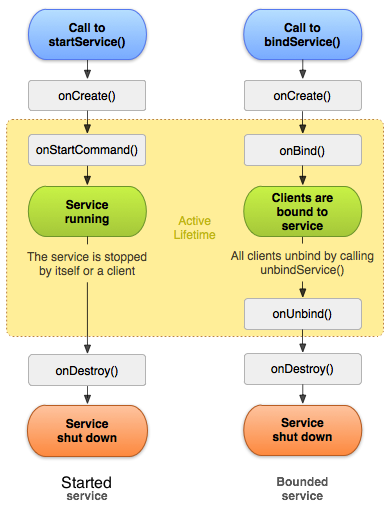
\includegraphics[scale=0.7]{service-lifecycle}

안드로이드 개발자 사이트의 그림에서는 Unbound Service와 Bound Service로 구분하였지만, Unbound Service는 혼동스런 용어이다. Bound되었다가 해제된 것을 의미한다고 오해할 수도 있기 때문에 Unbound Service보다는 Started Service로 부르는 게 더 맞겠다. 이 책에서도 이후 Started Service와 Bound Service로 언급하기로 한다.\\

Service는 보통 Started Service 또는 Bound Service로 존재하는데, Started이면서 Bound일 수도 있다.  Started \& Bound Service는 코드도 좀 더 복잡해지고 고려할 것이 두 배 이상이 되기 때문에 일반적으로 권장되지는 않는다. 가능하면 이런 시나리오는 배제하자.


